% GNUPLOT: LaTeX picture with Postscript
\begingroup
\newcommand{\ft}[0]{\footnotesize}
  \makeatletter
  \providecommand\color[2][]{%
    \GenericError{(gnuplot) \space\space\space\@spaces}{%
      Package color not loaded in conjunction with
      terminal option `colourtext'%
    }{See the gnuplot documentation for explanation.%
    }{Either use 'blacktext' in gnuplot or load the package
      color.sty in LaTeX.}%
    \renewcommand\color[2][]{}%
  }%
  \providecommand\includegraphics[2][]{%
    \GenericError{(gnuplot) \space\space\space\@spaces}{%
      Package graphicx or graphics not loaded%
    }{See the gnuplot documentation for explanation.%
    }{The gnuplot epslatex terminal needs graphicx.sty or graphics.sty.}%
    \renewcommand\includegraphics[2][]{}%
  }%
  \providecommand\rotatebox[2]{#2}%
  \@ifundefined{ifGPcolor}{%
    \newif\ifGPcolor
    \GPcolortrue
  }{}%
  \@ifundefined{ifGPblacktext}{%
    \newif\ifGPblacktext
    \GPblacktextfalse
  }{}%
  % define a \g@addto@macro without @ in the name:
  \let\gplgaddtomacro\g@addto@macro
  % define empty templates for all commands taking text:
  \gdef\gplbacktext{}%
  \gdef\gplfronttext{}%
  \makeatother
  \ifGPblacktext
    % no textcolor at all
    \def\colorrgb#1{}%
    \def\colorgray#1{}%
  \else
    % gray or color?
    \ifGPcolor
      \def\colorrgb#1{\color[rgb]{#1}}%
      \def\colorgray#1{\color[gray]{#1}}%
      \expandafter\def\csname LTw\endcsname{\color{white}}%
      \expandafter\def\csname LTb\endcsname{\color{black}}%
      \expandafter\def\csname LTa\endcsname{\color{black}}%
      \expandafter\def\csname LT0\endcsname{\color[rgb]{1,0,0}}%
      \expandafter\def\csname LT1\endcsname{\color[rgb]{0,1,0}}%
      \expandafter\def\csname LT2\endcsname{\color[rgb]{0,0,1}}%
      \expandafter\def\csname LT3\endcsname{\color[rgb]{1,0,1}}%
      \expandafter\def\csname LT4\endcsname{\color[rgb]{0,1,1}}%
      \expandafter\def\csname LT5\endcsname{\color[rgb]{1,1,0}}%
      \expandafter\def\csname LT6\endcsname{\color[rgb]{0,0,0}}%
      \expandafter\def\csname LT7\endcsname{\color[rgb]{1,0.3,0}}%
      \expandafter\def\csname LT8\endcsname{\color[rgb]{0.5,0.5,0.5}}%
    \else
      % gray
      \def\colorrgb#1{\color{black}}%
      \def\colorgray#1{\color[gray]{#1}}%
      \expandafter\def\csname LTw\endcsname{\color{white}}%
      \expandafter\def\csname LTb\endcsname{\color{black}}%
      \expandafter\def\csname LTa\endcsname{\color{black}}%
      \expandafter\def\csname LT0\endcsname{\color{black}}%
      \expandafter\def\csname LT1\endcsname{\color{black}}%
      \expandafter\def\csname LT2\endcsname{\color{black}}%
      \expandafter\def\csname LT3\endcsname{\color{black}}%
      \expandafter\def\csname LT4\endcsname{\color{black}}%
      \expandafter\def\csname LT5\endcsname{\color{black}}%
      \expandafter\def\csname LT6\endcsname{\color{black}}%
      \expandafter\def\csname LT7\endcsname{\color{black}}%
      \expandafter\def\csname LT8\endcsname{\color{black}}%
    \fi
  \fi
  \setlength{\unitlength}{0.0500bp}%
  \begin{picture}(8502.00,3968.00)%
    \gplgaddtomacro\gplbacktext{%
      \colorrgb{0.50,0.50,0.50}%
      \put(682,1173){\makebox(0,0)[r]{\strut{} 1}}%
      \colorrgb{0.50,0.50,0.50}%
      \put(682,1594){\makebox(0,0)[r]{\strut{} 2}}%
      \colorrgb{0.50,0.50,0.50}%
      \put(682,2016){\makebox(0,0)[r]{\strut{} 3}}%
      \colorrgb{0.50,0.50,0.50}%
      \put(682,2438){\makebox(0,0)[r]{\strut{} 4}}%
      \colorrgb{0.50,0.50,0.50}%
      \put(682,2860){\makebox(0,0)[r]{\strut{} 5}}%
      \colorrgb{0.50,0.50,0.50}%
      \put(682,3281){\makebox(0,0)[r]{\strut{} 6}}%
      \colorrgb{0.50,0.50,0.50}%
      \put(682,3703){\makebox(0,0)[r]{\strut{} 7}}%
      \colorrgb{0.50,0.50,0.50}%
      \put(861,484){\makebox(0,0){\strut{}4}}%
      \colorrgb{0.50,0.50,0.50}%
      \put(1263,484){\makebox(0,0){\strut{}9}}%
      \colorrgb{0.50,0.50,0.50}%
      \put(1666,484){\makebox(0,0){\strut{}16}}%
      \colorrgb{0.50,0.50,0.50}%
      \put(2068,484){\makebox(0,0){\strut{}25}}%
      \colorrgb{0.50,0.50,0.50}%
      \put(2471,484){\makebox(0,0){\strut{}36}}%
      \colorrgb{0.50,0.50,0.50}%
      \put(2873,484){\makebox(0,0){\strut{}49}}%
      \colorrgb{0.50,0.50,0.50}%
      \put(3276,484){\makebox(0,0){\strut{}64}}%
      \colorrgb{0.50,0.50,0.50}%
      \put(3678,484){\makebox(0,0){\strut{}81}}%
      \colorrgb{0.50,0.50,0.50}%
      \put(4081,484){\makebox(0,0){\strut{}100}}%
      \colorrgb{0.50,0.50,0.50}%
      \put(4483,484){\makebox(0,0){\strut{}121}}%
      \colorrgb{0.50,0.50,0.50}%
      \put(4885,484){\makebox(0,0){\strut{}144}}%
      \colorrgb{0.50,0.50,0.50}%
      \put(5288,484){\makebox(0,0){\strut{}169}}%
      \colorrgb{0.50,0.50,0.50}%
      \put(5690,484){\makebox(0,0){\strut{}196}}%
      \colorrgb{0.50,0.50,0.50}%
      \put(6093,484){\makebox(0,0){\strut{}225}}%
      \colorrgb{0.50,0.50,0.50}%
      \put(6495,484){\makebox(0,0){\strut{}256}}%
      \colorrgb{0.50,0.50,0.50}%
      \put(6898,484){\makebox(0,0){\strut{}289}}%
      \colorrgb{0.50,0.50,0.50}%
      \put(7300,484){\makebox(0,0){\strut{}324}}%
      \colorrgb{0.50,0.50,0.50}%
      \put(7703,484){\makebox(0,0){\strut{}400}}%
      \colorrgb{0.50,0.50,0.50}%
      \put(8105,484){\makebox(0,0){\strut{}441}}%
      \csname LTb\endcsname%
      \put(176,2227){\rotatebox{-270}{\makebox(0,0){\strut{}Przyspieszenie S}}}%
      \put(4483,154){\makebox(0,0){\strut{}Liczba procesów}}%
    }%
    \gplgaddtomacro\gplfronttext{%
      \csname LTb\endcsname%
      \put(7118,3530){\makebox(0,0)[r]{\strut{}Cannon}}%
      \csname LTb\endcsname%
      \put(7118,3310){\makebox(0,0)[r]{\strut{}MKL}}%
    }%
    \gplbacktext
    \put(0,0){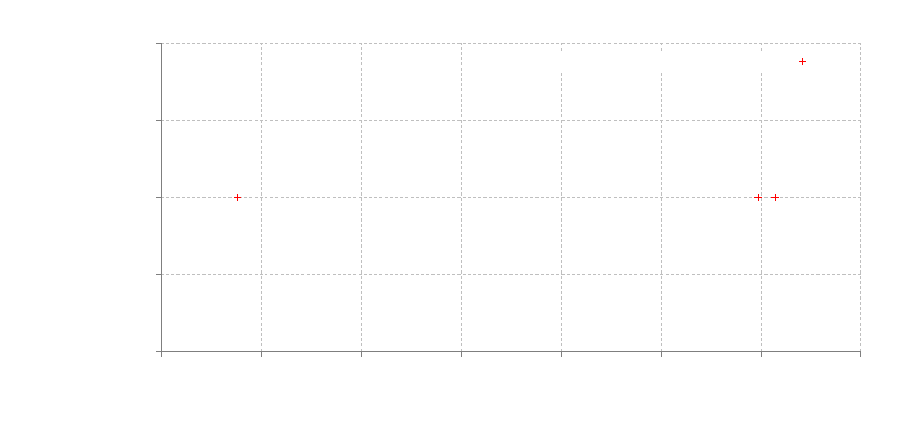
\includegraphics{speedup}}%
    \gplfronttext
  \end{picture}%
\endgroup
